
\begin{questions}
\question{
Volume of an n-ball and area of an n-sphere
}
\begin{solution}
  To compute the volume of an n-ball ($\mathcal{B}$) we can begin by setting the integral
  \begin{equation}
    V_n(R) = \int_{\mathcal{B}} dx_1dx_2\ldots dx_n = \alpha_nR^n.
    \label{vol:1}
  \end{equation}
  We know by dimensional analysis that the dimensions of the volume of the n-ball must be $R$, hence there must be a factor $R^n$ embedded in the final result, times some factor dependent of n.
  The surface of an n-sphere will be denoted by $S_{n-1}(R)$. We can also obtain the volume of the n-ball, if we integrate very thin spherical shells of radius $r\in[0,R]$. This idea is represented by the following equation \begin{equation}
    V_n(R) = \int_0^R S_{n-1}(r)dr.
    \label{vol:2}
  \end{equation}
  If we integrate this equation and rember that on $r=0$ the sphere must have area $0$, we have
  \begin{equation}
    S_{n-1}(R = \frac{dV_n(R)}{dR} = n\alpha_nR^{n-1}, \text{ using eq. \ref{vol:1}.}
    \label{surf:1}
  \end{equation}
  So, as we can see, our original problem is now reduced to find the functional form of $\alpha_n$. To gain insight let's look at what happens if we combine eqs. \ref{vol:1}-\ref{surf:1}.
  \begin{equation}
    \int_{\mathcal{B}} dx_1dx_2\ldots dx_n = \int_0^R S_{n-1}(r)dr = n\alpha_n\int_0^R r^{n-1} dr.
    \label{vol:3}
  \end{equation}
  Now let's do two things. First, we need to realize that on the right hand side of eq. \ref{vol:3} there are two parts, one exclusively dependent on $n$ and another dependent on $n,r$ (the integral). Knowing this let's take our second step and express the volume element $dx_1dx_2\ldots dx_n$ in spherical coordinates. Therefore, it will look like this
  \begin{equation}
    dx_1dx_2\ldots dx_n = r^{n-1}drd\Omega_{n-1},
  \end{equation}
  where $d\Omega$ is the element of solid angle. From here we can conclude that
  \begin{equation}
    \int_{\Omega} d\Omega_{n-1} = n\alpha_n.
    \label{om:alp}
  \end{equation}

  Here we need an auxiliary result. Let's calculate $\Gamma(1/2)$ from the definition
  \begin{equation}
    \begin{aligned}[b]
      \Gamma \left(\frac{1}{2} \right) &= \int_0^\infty \exp(-t)t^{(1/2 - 1)}dt, \quad\textnormal{  changing $t = x^2$ }.\\
      &= \int_0^\infty \exp(-x^2)x^{-1} 2xdx,\\
      &= 2 \int_0^\infty \exp(-x^2)dx, \\
      & =\int_{-\infty}^\infty \exp(-x^2)dx,\\
      & = \sqrt{\pi}.
    \end{aligned}
  \end{equation}
  Now let's play with this idea
  \begin{equation}
    \exp(-(x_1^2 +x_2^2 + \cdots + x_n^2)) = \exp{(-r^2)}.
    \label{exp:radial}
  \end{equation}
  Which is just expressing the same function in two different coordinate systems. What would happen is we integrate such functions over all space?
  \begin{equation}
    \int_{-\infty}^\infty \cdots \int_{-\infty}^\infty \exp(-(x_1^2 +x_2^2 + \cdots + x_n^2)) dx_1dx_2\ldots dx_n = \int_{0}^\infty r^{n-1}dr \int_\Omega d\Omega_{n-1} \exp{(-r^2)}.
  \end{equation}
  With our previous knowledge from eq. \ref{om:alp} and integral calculus we can do this
  \begin{equation}
    \int_{-\infty}^\infty \exp{(-x_1^2)}dx_1\cdots \int_{-\infty}^\infty \exp{(-x_n^2)}dx_n = \int_{0}^\infty r^{n-1}dr \int_\Omega d\Omega_{n-1} \exp{(-r^2)}.
  \end{equation}
  Using eq. \ref{om:alp}
  \begin{equation*}
    \int_{-\infty}^\infty \exp{(-x_1^2)}dx_1\cdots \int_{-\infty}^\infty \exp{(-x_n^2)}dx_n = n\alpha_n\int_{0}^\infty r^{n-1}dr \exp{(-r^2)}.
  \end{equation*}
  On the left hand side we have $n$ times $\Gamma(1/2)$. But we already know their value, hence
  \begin{equation}
    \int_{-\infty}^\infty \exp{(-x_1^2)}dx_1\cdots \int_{-\infty}^\infty \exp{(-x_n^2)}dx_n = (\sqrt{\pi})^n.
  \end{equation}
  And from the definition of $\Gamma$ we know
  \begin{equation}
    \int_0^\infty r^{n-1}\exp{(-r^2)} dr = \frac{1}{2} \Gamma \left(\frac{n}{2}\right).
  \end{equation}
  And as a consequence,
  \begin{equation*}
    \begin{aligned}[b]
      \pi^{n/2} &= \alpha_n \frac{n}{2} \Gamma \left(\frac{n}{2}\right),\\
      & = \alpha_n \Gamma \left(\frac{n}{2} + 1 \right).
    \end{aligned}
  \end{equation*}
  Hence
  \begin{equation}
    \alpha_n = \frac{\pi^{n/2}}{\Gamma \left(\frac{n}{2} + 1 \right)}.
  \end{equation}
  Now, substituting this on eqs. \ref{vol:1} and \ref{surf:1} we have

  \begin{equation}
    \hlgreen{V_n(R) = \frac{\pi^{n/2}R^n}{\Gamma \left(\frac{n}{2} + 1 \right)}.}
  \end{equation}
  \begin{equation*}
    S_{n-1}(R) = \frac{n\pi^{n/2}R^{n-1}}{\Gamma \left(\frac{n}{2} + 1 \right)}.
  \end{equation*}
  Using the property $\Gamma(s+1) = s\Gamma(s)$ we can modify this last equation to get finally
  \begin{equation}
    \hlgreen{S_{n-1}(R) = \frac{2\pi^{n/2}R^{n-1}}{\Gamma \left(\frac{n}{2}\right)}.}
  \end{equation}
 \end{solution}
 \clearpage

 \question{Density of states of a n-dimensional free electron gas}
 \begin{solution}
   At this point we are already quite acquainted with integrals in n dimensional spaces. The next step is now, taking all that knowledge and put it to work. How? We will see that in the present section.

   Suppose we want to know the number of states $N$ inside an n-dimensional ball in $k-$space. A quick way to calculate this would be to take the entire volume of the ball and divide it by the volume each state occupies. Sounds reasonable, let's proceed with this idea in form of equations
   \begin{equation}
     N = \frac{V_n(k)}{V_{state}}
   \end{equation}
   From the last section we already know the volume of an n-ball. But do we know the volume occupied by a state in the $k-$space? Sure we know, that volume is our friend the volume of the Brillouin zones $V_state = (2\pi)^n/V$, where V is the volume of the direct cell, and we should not be extremely worried by it, we will see why is that the case.

   By the above arguments we arrive to this

   \begin{equation}
     N = \frac{2\pi^{n/2}k_\epsilon^n}{\Gamma\left(\frac{n}{2} + 1\right)(2\pi)^n/V} =  \frac{2\pi^{n/2}(2m\epsilon/\hbar^2)^{n/2}}{\Gamma\left(\frac{n}{2} + 1\right)(2\pi)^n}V.
     \label{N}
   \end{equation}
Where we have use the fact that
\begin{equation}
  k^2_\epsilon = \left(\frac{2m\epsilon}{\hbar^2}\right)^n
\end{equation}
So the number of states per volume in the direct cell is
\begin{equation}
  n = \frac{N}{V} =   \frac{2\pi^{n/2}(2m\epsilon/\hbar^2)^{n/2}}{\Gamma\left(\frac{n}{2} + 1\right)(2\pi)^n}.
  \label{N}
\end{equation}
We can now proceed to compute the density of states $D(\epsilon) = dn/d\epsilon$.
\begin{equation}
  \begin{aligned}[b]
    D(\epsilon) &= dn/d\epsilon,\\
    &= \frac{2\pi^{n/2}(2m/\hbar^2)^{n/2}}{\Gamma\left(\frac{n}{2} + 1\right)(2\pi)^n} \frac{d}{d\epsilon} (\epsilon)^{n/2},\\
    &= \hlgreen{\frac{2\pi^{n/2}(2m/\hbar^2)^{n/2}}{\Gamma\left(\frac{n}{2} + 1\right)(2\pi)^n} \frac{n}{2} (\epsilon)^{n/2 -1}.}
  \end{aligned}
\end{equation}
If we use this formula we will obtain for the cases when $n=1,2,3$

\begin{eqnarray}
  &D_1(\epsilon) = \frac{\sqrt{2m/\hbar^2}}{\pi}\epsilon^{-1/2},\\
  &D_2(\epsilon) = \frac{m}{\pi\hbar^2},\\
  &D_3(\epsilon) = \frac{1}{2\pi^2}\left(\frac{2m}{\hbar^2}\right)^{3/2}(\epsilon)^{1/2}.
\end{eqnarray}
The plots of this equations can be found in fig. \ref{dos}. And as we can see, they agree with what we saw in class.
\begin{center}
  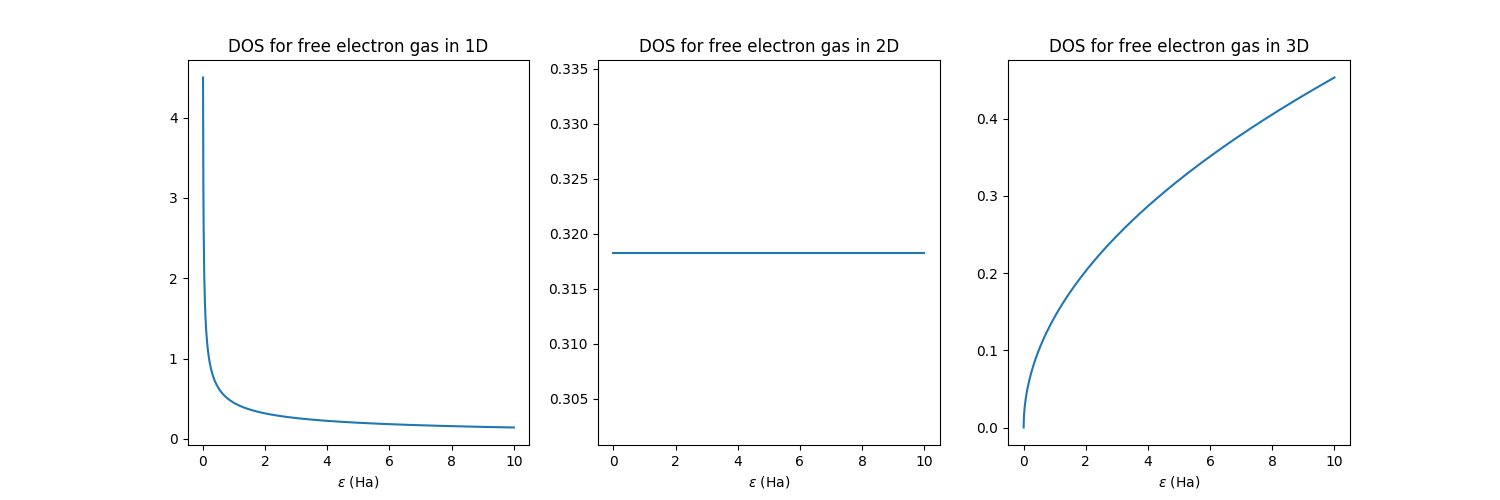
\includegraphics[width=\linewidth]{Dos.png}
\end{center}
\captionof{figure}{Density of states for 1D, 2D, and 3D.}\label{dos}\vspace{0.5cm}

 \end{solution}

 \question{Fermi energy}

 \begin{solution}
   We will begin this exercise by commenting that a hyper-sphere can be divided into $2^n$ congruent hyperoctants. We also know that the energy of a state labeled by $n_i, i=1,2,\ldots,n$, in a cubical box, is given by
   \begin{equation}
     E_{\vec{n}} = \frac{\hbar^2\pi^2}{2mL^2}(n_1^2+n_2^2+\cdots+n_n^2).
   \end{equation}
   We can just represent this with the norm of a vector $\vec{n}$ like
   \begin{equation}
     E_{\vec{n}} = \frac{\hbar^2\pi^2}{2mL^2}|\vec{n}|.
     \label{ene}
   \end{equation}
   The number of states with energy less than $E_F$ is equal to the number of states that lie within a sphere of radius $\vec{n}_F$ in the region of n-space where all the $n_i>0$, hence
   \begin{equation}
     N = 2\times \frac{1}{2^n}\times \frac{\pi^{n/2}n_F^n}{\Gamma \left(\frac{n}{2} + 1 \right)},
   \end{equation}
   Where the first factor 2 comes from the fact that we have two opposite spins for every state, the $1/2^n$ corresponds to the hyper-octant of the n-ball with all $n_i>0$.

   Therefore
   \begin{equation}
     n_F =  \left(\frac{2^{n-1}N\Gamma \left(\frac{n}{2} + 1 \right)}{\pi^{n/2}} \right)^{1/n}.
   \end{equation}
   When we plug this last equation into eq. \ref{ene} we will obtain the Fermi energy
   \begin{equation}
     E_F = \frac{\hbar^2\pi^2}{2mL^2}\left(\frac{2^{n-1}N\Gamma \left(\frac{n}{2} + 1 \right)}{\pi^{n/2}} \right)^{2/n},
   \end{equation}
   If we get $L$ into the expression between parenthesis we'll have
   \begin{equation}
     E_F = \frac{\hbar^2\pi}{2m}\left(\frac{2^{n-1}N\Gamma \left(\frac{n}{2} + 1 \right)}{L^n} \right)^{2/n},
   \end{equation}
   but $N/L^n = \rho$, therefore
   \begin{equation}
     \hlgreen{E_F(\rho) = \frac{\hbar^2\pi}{2m}\left(2^{n-1}\Gamma \left(\frac{n}{2} + 1 \right) \right)^{2/n}\rho ^{2/n}.}
   \end{equation}
   If we try this formula for 2D we get
\begin{equation}
  \begin{aligned}[b]
    E_F &= \frac{\hbar^2\pi}{2m}\left(2^{2-1}\Gamma \left(\frac{2}{2} + 1 \right) \right)^{2/2}\rho ^{2/2},\\
    &=\frac{\hbar^2\pi}{2m}\left(2\Gamma \left(2 \right) \right)\rho,\\
    &=\frac{\hbar^2\pi}{m}\rho.
  \end{aligned}
\end{equation}
In 3D we get
\begin{equation}
  \begin{aligned}[b]
    E_F(\rho) &= \frac{\hbar^2\pi}{2m}\left(2^{3-1}\Gamma \left(\frac{3}{2} + 1 \right) \right)^{2/3}\rho ^{2/3},\\
    &= \frac{\hbar^2\pi}{2m}\left(4\Gamma \left(\frac{5}{2} \right) \right)^{2/3}\rho ^{2/3},\\
    &= \frac{\hbar^2\pi}{2m}\left(4 \left(\frac{3}{4}\sqrt{\pi} \right) \right)^{2/3}\rho ^{2/3},\\
    &= \frac{\hbar^2\pi}{2m}\left(3\sqrt{\pi}  \right)^{2/3}\rho ^{2/3},\\
    &= \frac{\hbar^2\pi}{2m}\left(3\sqrt{\pi} (\pi)^{3/2} \right)^{2/3}\rho ^{2/3},\\
    &= \frac{\hbar^2\pi}{2m}\left(3\pi^{2} \right)^{2/3}\rho ^{2/3},
  \end{aligned}
\end{equation}
  Both results agree with the results we already had for 2D and 3D.
 \end{solution}

\end{questions}

%
% \begin{center}
%   \includegraphics[width=55mm]{}
% \end{center}
%
% \captionof{figure}{}\label{new}\vspace{0.5cm}
